\documentclass{article}
\usepackage{tikz}
\usepackage{amsmath}
\usepackage[paperwidth=34cm,paperheight=18cm,margin=8mm]{geometry}
\usetikzlibrary{arrows.meta, positioning, fit, backgrounds, calc}

\definecolor{cIn}{HTML}{1F4E79}
\definecolor{cCell}{HTML}{B7472A}
\definecolor{cLoop}{HTML}{2E7D32}
\definecolor{cOut}{HTML}{6A1B9A}
\definecolor{cBg}{HTML}{F4F6F8}

\begin{document}
\thispagestyle{empty}
\centering
\vspace*{\fill}
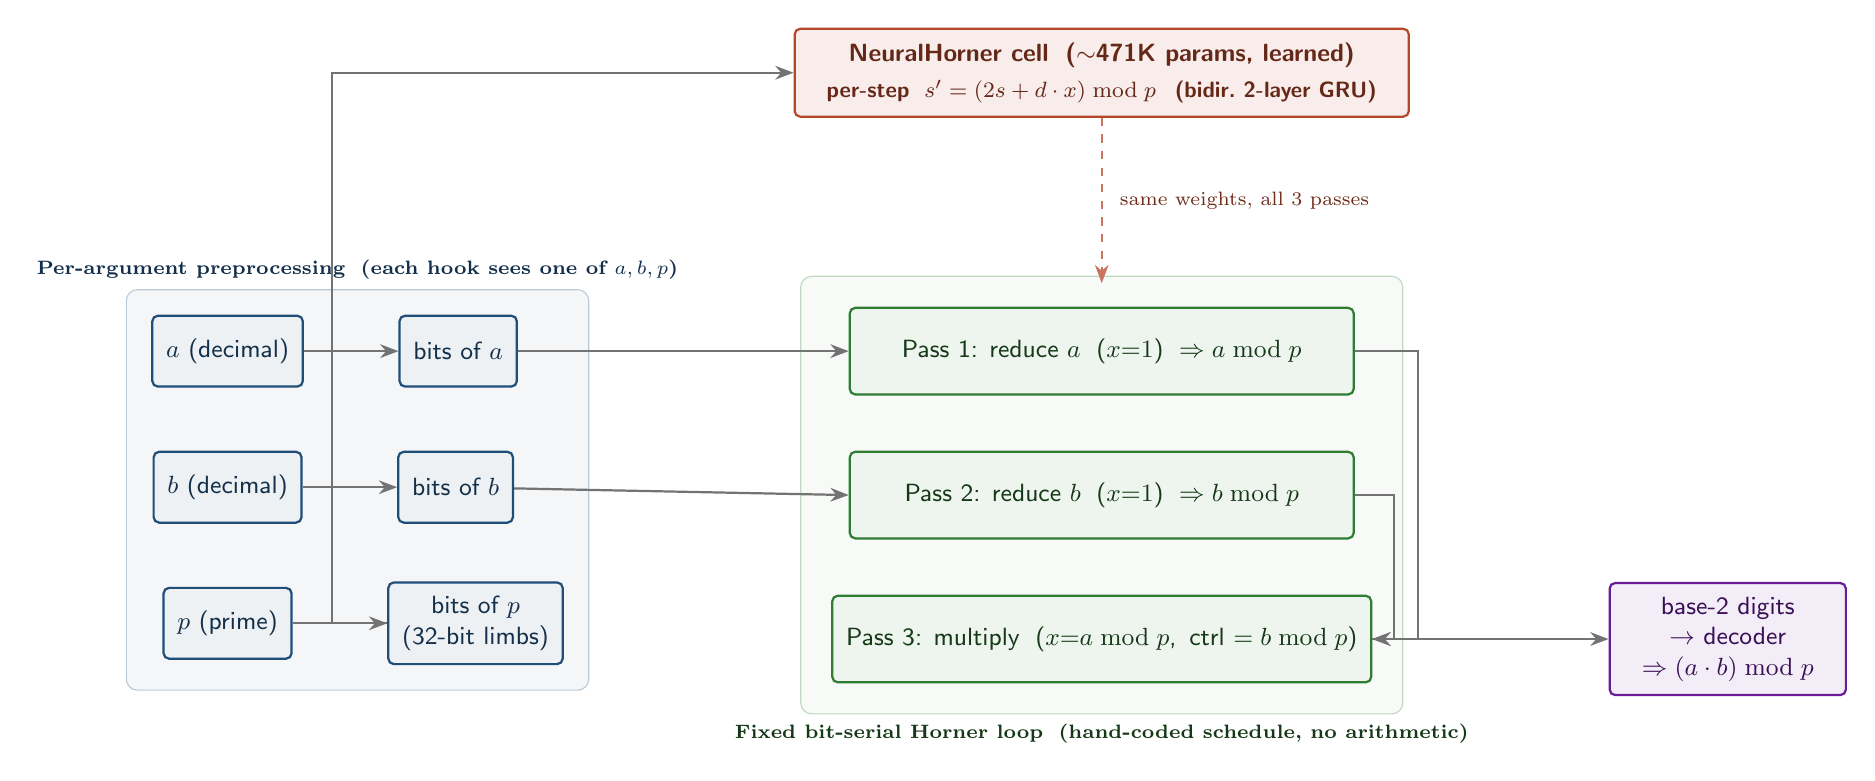
\begin{tikzpicture}[
  font=\sffamily\small, >=Stealth,
  box/.style={rounded corners=2pt, draw, thick, align=center, minimum height=9mm, inner sep=5pt},
  inn/.style={box, draw=cIn, fill=cIn!8, text=cIn!60!black},
  cell/.style={box, draw=cCell, fill=cCell!10, text=cCell!55!black, font=\sffamily\small\bfseries, minimum width=78mm},
  pass/.style={box, draw=cLoop, fill=cLoop!8, text=cLoop!45!black, minimum width=64mm, minimum height=11mm},
  outb/.style={box, draw=cOut, fill=cOut!8, text=cOut!55!black, minimum width=30mm},
  flow/.style={->, thick, draw=black!55},
  share/.style={->, dashed, thick, draw=cCell!75},
]

% column 1 inputs ; column 2 bits
\node[inn] (a) {$a$ (decimal)};
\node[inn, below=8mm of a] (b) {$b$ (decimal)};
\node[inn, below=8mm of b] (p) {$p$ (prime)};
\node[inn, right=12mm of a] (ab) {bits of $a$};
\node[inn, right=12mm of b] (bb) {bits of $b$};
\node[inn, right=12mm of p] (pb) {bits of $p$\\(32-bit limbs)};
\draw[flow] (a)--(ab); \draw[flow] (b)--(bb); \draw[flow] (p)--(pb);

% column 3 the three passes, stacked
\node[pass, right=42mm of ab] (r1) {Pass 1: reduce $a$ \;($x{=}1$)\; $\Rightarrow a\bmod p$};
\node[pass, below=7mm of r1] (r2) {Pass 2: reduce $b$ \;($x{=}1$)\; $\Rightarrow b\bmod p$};
\node[pass, below=7mm of r2] (m)  {Pass 3: multiply \;($x{=}a\bmod p$,\, ctrl $=b\bmod p$)};
\draw[flow] (ab) -- (r1.west);
\draw[flow] (bb) -- (r2.west);
\draw[flow] (r1.east) -- ++(8mm,0) |- (m.east);
\draw[flow] (r2.east) -- ++(5mm,0) |- (m.east);

% column 4 output
\node[outb, right=30mm of m] (o) {base-2 digits\\ $\to$ decoder\\ $\Rightarrow (a\cdot b)\bmod p$};
\draw[flow] (m.east) -- (o.west);

% shared cell, centered well ABOVE the loop; one clean dashed link into the gap
\node[cell, above=24mm of r1] (cell) {NeuralHorner cell \;($\sim$471K params, learned)\\[2pt]
  \footnotesize per-step\; $s' = (2s + d\cdot x)\bmod p$ \;\,(bidir.\ 2-layer GRU)};
\draw[share] (cell.south) -- node[right=1mm, font=\scriptsize, text=cCell!60!black]
  {same weights, all 3 passes} ($(r1.north)+(0,3mm)$);
% modulus conditioning routed up the left gap, around the boxes
\draw[flow] (pb.west) -- ++(-7mm,0) |- ($(cell.west)+(-12mm,0)$) -- (cell.west);

\begin{scope}[on background layer]
  \node[fit=(a)(pb), rounded corners, fill=cBg, draw=cIn!30, inner sep=9pt,
    label={[cIn!60!black,font=\scriptsize\bfseries]above:Per-argument preprocessing \;(each hook sees one of $a,b,p$)}] {};
  \node[fit=(r1)(m), rounded corners, fill=cLoop!4, draw=cLoop!30, inner sep=11pt,
    label={[cLoop!45!black,font=\scriptsize\bfseries]below:Fixed bit-serial Horner loop \;(hand-coded schedule, no arithmetic)}] {};
\end{scope}

\end{tikzpicture}
\vspace*{\fill}
\end{document}
